\section{Target audience analysis}\label{sec:target-audience-analysis}

When working on a large scale project, it is important to ask ourselves ``who are we doing this for?''.
The problem has to be big enough to affect a big number of users and the solution has to be viable to be used by said
users.
But we can't make a solution without understanding who our users are.

\subsection{Audience}\label{subsec:audience}

Our concern is about travelling, which covers a wide range of people, as everyone travels one way or another.
Some examples include travelling to work, to school, family visits, or outings with friends.
Therefore, we have to narrow it down, as we can't address everyone.
There are already some solution to that issue, but from our `analysis over existing solutions', we figured that they are
more fit for single trips, rather than every day travelling.
This is mainly what we want to focus on, which is why our target audience is \underline{commuters}.

\subsection{Age range}\label{subsec:age-range}

With our group in mind, we can estimate an age range for commuters.
Commuting means to travel to the same destination and back on a regular basis.
Therefore, our focus on destinations for commuting are either education or work.

In Denmark, primary schools are picked based on the district where the student lives~\cite{primary_school}.
This would exclude them from our target audience, because we want to focus on long distance commuters.
At shorter distances, we would need to exclude planes, trains, and for people younger than 18, cars, making it a matter
of whether the student should commute by walking or by bike, which are both \unit{CO_{2}} friendly options.
This makes our solution irrelevant for this age group.
Things change from secondary education however, as students can freely pick which high school they want to go to.
This makes them a better candidate for our problem, as they can choose a school farther away from where they live.
Secondary education starts when the student is 16 years old~\cite{secondary_school}.
Our cutoff in the age range would be retirement.
We looked into when the retirement age is in Denmark, and it is 66--68 years of age~\cite{retirement}.
That would make our age range \underline{between 15 and 68 years}.

The age range is quite big compared to many other projects, which makes our solution rather difficult, as we have to
accommodate it for teenagers, adults and elderly.
This would mean to make the program both easy and fast to use.

\subsection{Sender}\label{subsec:sender}

As this is a private project, the sender is us.
Rejseplanen, which is a similar solution that we've been looking inspiration from, is owned by DSB, Movia and many
others from the public transportation business~\cite{om_rejseplanen}, so if we were tasked by them to make a solution to
the main problem, then they would be the senders.
However, we're not looking to distribute our program.

\subsection{Persona}\label{subsec:persona}

To further analyze our age group, we decided to use the \textit{persona} method.
How it works is that we create fictional people with different issues and look into how our solution could help them
with their issue.
We have made 3 personas, where each of them cover different age groups and have distinct characteristics related to the
main problem.

\renewcommand{\arraystretch}{1.5}

\begin{tabularx}{\textwidth}{ | l X | }
    \hline
    &                                                      \\
    & 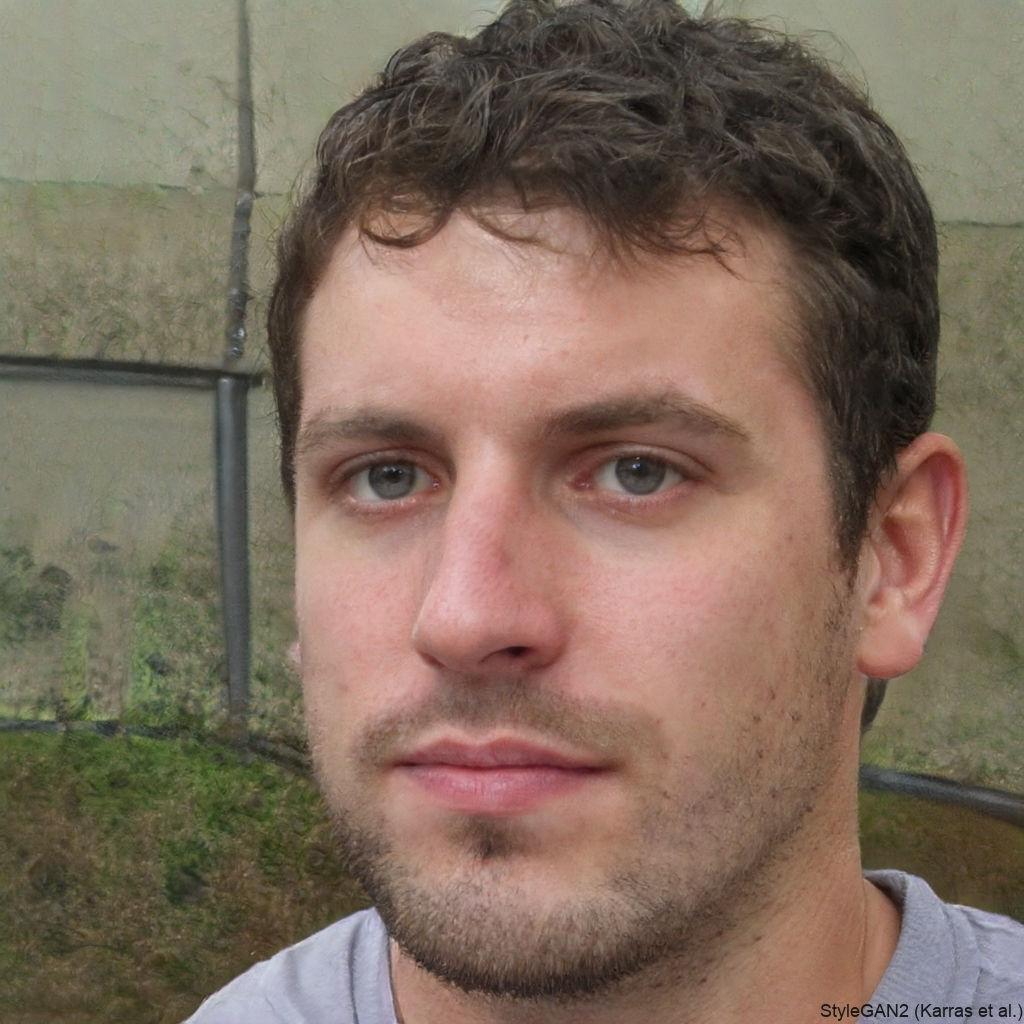
\includegraphics[width=0.25\textwidth]{images/asger} \\
    Name       & Asger Johansen                                       \\
    Age        & 28 years old                                         \\
    Occupation & Designer                                             \\
    What's important & For Asger it is important to spend his days to the fullest.
    He is very outgoing, so he goes out with people after work.
    He hates having to stay overtime. \\
    Current problem & Asger just got a new job offer, but it's in another city.
    He isn't sure whether to move out or to commute there.
    He is also afraid of losing his free time if he has to travel. \\
    Potential solution & We would want to make a program, where Asger could calculate how long it'd take to commute from
    where he lives to the new job.
    He could compare different forms of transport and decide whether it's worth it to commute or if he should move out
    instead. \\
    \hline
\end{tabularx}

\begin{tabularx}{\textwidth}{ | l X | }
    \hline
    &                                                         \\
    & 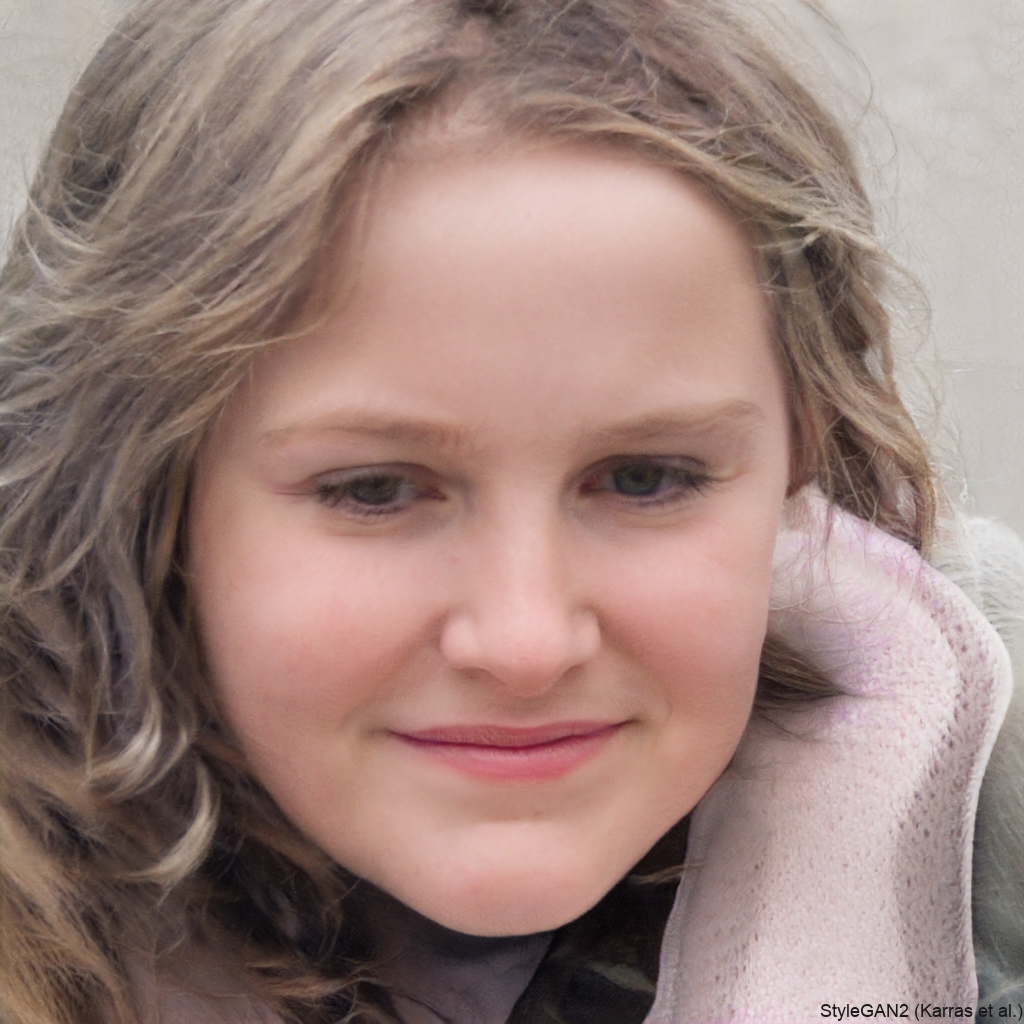
\includegraphics[width=0.25\textwidth]{images/josefine} \\
    Name       & Josefine Madsen                                         \\
    Age        & 19 years old                                            \\
    Occupation & Student                                                 \\
    What's important & For Josefine it is important to look after the nature.
    She's been taught to think green since she was little, so she doesn't like taking public transport and doesn't want
    to drive a gas car. \\
    Current problem & Josefine is starting university, but she lives outside the city.
    She is considering whether to take the S-train, the train or a bus to university.
    She is also considering buying an electric car. \\
    Potential solution & We would want to make a program, where Josefine could calculate how much the emissions is made
    from different forms of transport.
    She can then compare them and choose what works best for her. \\
    \hline
\end{tabularx}

\begin{tabularx}{\textwidth}{ | l X | }
    \hline
    &                                                       \\
    & 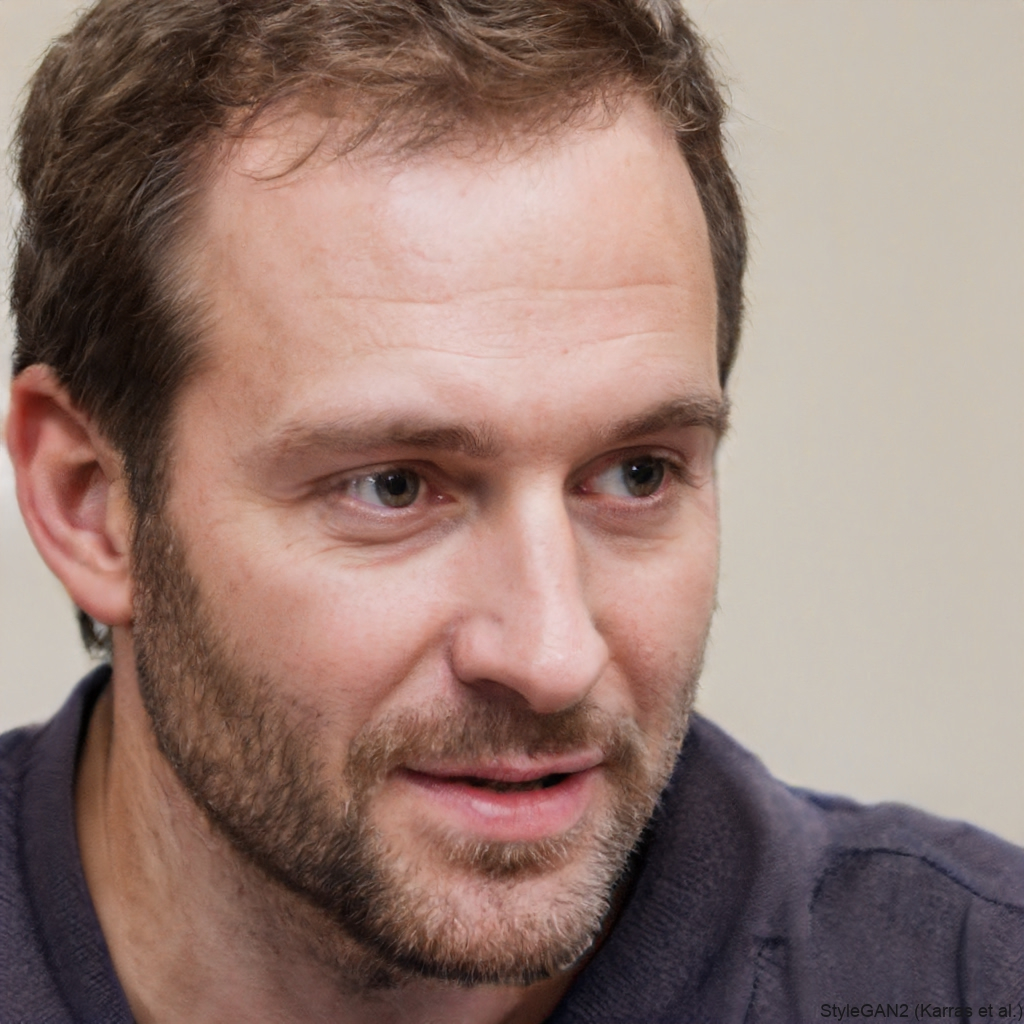
\includegraphics[width=0.25\textwidth]{images/martin} \\
    Name       & Martin Jensen                                         \\
    Age        & 34 years old                                          \\
    Occupation & Factory worker                                        \\
    What's important & For Martin it is important to live a carefree life.
    He has a family and friends at work, so he's pretty happy with himself. \\
    Current problem & Martin drives a gas car to work, but he wants to change that for the sake of the environment.
    He has gotten used to the comfort of his car, but can't afford an electric car.
    He wonders if public transport could match that. \\
    Potential solution & We would want to make a program, where Martin can figure out what forms of public transport are
    most comfortable and most climate friendly. \\
    \hline
\end{tabularx}
